% DAFN24 - Robotics - Lecture 9
% Roberto Masocco <roberto.masocco@uniroma2.it>
% June 5, 2024

\documentclass[aspectratio=169]{beamer}

% Slides layout
\usepackage[
    title={MARTe2},
    subtitle={A real-time control framework for nuclear fusion},
    event={DAFN},
    author={Roberto Masocco},
    longauthor={Roberto Masocco},
    email={roberto.masocco@uniroma2.it},
    institute={Tor Vergata},
    longinstitute={University of Rome Tor Vergata},
    department={Department of Civil Engineering and Computer Science Engineering},
    researchgroup={},
    date={June 12, 2024}
]{utvengbeamer}

% Code listings settings
\usepackage[nomath]{lmodern}
\definecolor{codegreen}{rgb}{0 0.5 0}
\definecolor{codered}{rgb}{1 0 0}
\definecolor{codeocher}{rgb}{0.8 0.47 0.13}
\usepackage{listings}
\newcommand{\listingsfont}{\ttfamily}
\lstdefinestyle{normal}{
    basicstyle=\ttfamily\small,
    commentstyle=\color{codegreen},
    breakatwhitespace=false,
    captionpos=b,
    frame=lines,
    keepspaces=true,
    keywordstyle=\color{codered}\bfseries,
    numbers=left,
    numbersep=5pt,
    numberstyle=\footnotesize,
    showspaces=false,
    showstringspaces=false,
    showtabs=false,
    stringstyle=\color{codeocher},
    tabsize=2
}
\lstdefinestyle{small}{
    basicstyle=\linespread{0.8}\ttfamily\small,
    commentstyle=\color{codegreen},
    breakatwhitespace=false,
    captionpos=b,
    frame=lines,
    keepspaces=true,
    keywordstyle=\color{codered}\bfseries,
    numbers=left,
    numbersep=5pt,
    numberstyle=\footnotesize,
    showspaces=false,
    showstringspaces=false,
    showtabs=false,
    stringstyle=\color{codeocher},
    tabsize=2
}
\lstdefinelanguage{cfg}{
  sensitive=true,
  keywords = [2]{Class, Functions, Data, States, Scheduler, Signals, InputSignals, OutputSignals, Parameters, DataSource, Type, Threads, CPUs, DefaultDataSource, SleepNature, TimingDataSource, NextState, NextStateError, Destination, Function, Library, SymbolPrefix},
  keywordstyle = [2]\color{codered},
  keywords =[3]{\$RTApp, GAM1, Input1, Output1, DDB1, Logger, Timings, Counter, Timer, Time, State1, Thread1, FSM, STATE1, STATE2, ERROR, GOTOSTATE1, GOTOSTATE2, PrepareChangeToState2Msg, StopCurrentStateExecutionMsg, StartNextStateExecutionMsg, GAMGain, Input1, Output1, Param1},
  keywordstyle = [3]\color{blue},
  keywords =[4]{PrepareNextState, StopCurrentStateExecution, StartNextStateExecution, Gain},
  keywordstyle = [4]\color{cyan},
  morecomment=[l][\color{codegreen}]{\//}
}

\begin{document}

% --- Title page ---
\frame{\titlepage}

% --- Table of contents ---
\begin{frame}
    \frametitle{Roadmap}
    \tableofcontents
\end{frame}

% --- Section 1 ---
% Section 1 - Introduction
% Alessandro Tenaglia <alessandro.tenaglia@uniroma2.it>
% May 6, 2022

% ### Introduction ###
\section{Introduction}
\graphicspath{{figs/section1/}}

% --- Overview ---
\begin{frame}{Overview}
	\begin{block}{Multi-threaded Application Real-Time executor}
		MARTe is a \textbf{C++ modular} and \textbf{multi-platform framework} for the development of \textbf{multi-threaded real-time control system applications}.
	\end{block}
\end{frame}

% --- MARTe1 ---
\begin{frame}{MARTe1}
	\begin{columns}
		\column{.5\textwidth}
		\begin{itemize}
			\item \textbg{MARTe1} is the previous version of this framework;
			\item \textbg{MARTe1} was deployed in many fusion real-time control systems, i.e. JET tokamak;
			\item The use of \textbg{MARTe1} increased the number of supported environments and platforms;
		\end{itemize}
		\column{.5\textwidth}
		\begin{figure}
			\centering
			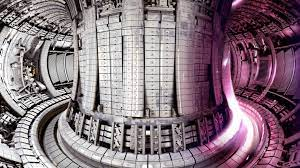
\includegraphics[scale=.5]{JET.jpeg}
			\label{fig:jet}
			\caption{JET Tokamak}
		\end{figure}
	\end{columns}
\end{frame}


% --- Section 2 ---
% Section 2 - Core library
% Alessandro Tenaglia <alessandro.tenaglia@uniroma2.it>
% May 6, 2022

% ### Core library ###
\section{Core library}
\graphicspath{{figs/section2/}}

% --- Code organisation ---
\begin{frame}{Code organisation}
	One of the main features of the MARTe2 architecture is the bold separation between:
	\begin{itemize}
		\item<1-> the platform \textbg{architecture}, i.e. x86, armv8;
		\item<2-> the \textbg{environment} details, i.e. Linux, FreeRTOS, Windows;
		\item<3-> the \textbg{real-time algorithms}, i.e. the user code;
	\end{itemize}
\end{frame}

% --- Code organisation ---
\begin{frame}{Code organisation}
	\begin{figure}
		\centering
		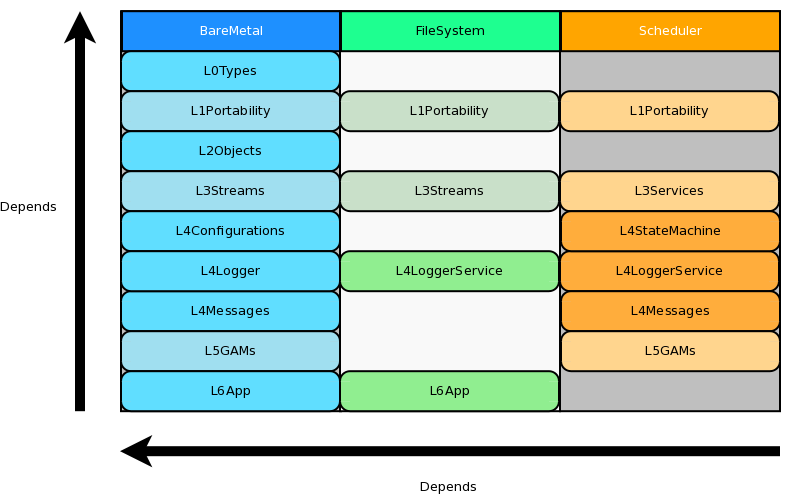
\includegraphics[scale=.35]{Tiers.png}
		\label{fig:tiers}
		\caption{Code library}
	\end{figure}
\end{frame}

% --- Makefile ---
\begin{frame}{Makefile}
	\begin{columns}
		\column{.5\textwidth}
		The build of the core library (and all MARTe2 base projects) follows this structure:
		\begin{itemize}
			\item<1-> The \textbg{Makefile.os-arch} defines the \textbg{TARGET} operating system and architecture;
			\item<2-> The \textbg{Makefile.inc} defines all the common rules;
			\item<3-> The \textbg{MakeDefaults} defines the specific rules for the \textbg{TARGET};
		\end{itemize}
		\column{.5\textwidth}
		\begin{figure}
			\centering
			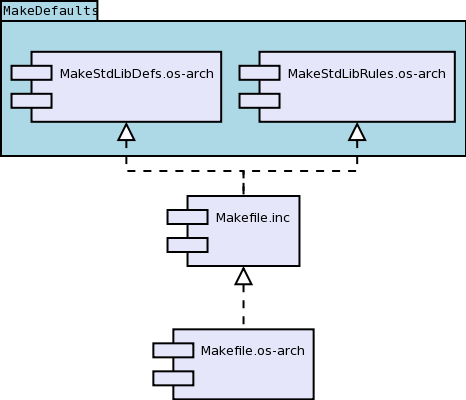
\includegraphics[scale=.3]{Makefiles.png}
			\label{fig:makefiles}
			\caption{Makefile structure, \\ from bottom to top}
		\end{figure}
	\end{columns}
\end{frame}


% --- Section 3 ---
% Section 3 - Real-Time Applications
% Alessandro Tenaglia <alessandro.tenaglia@uniroma2.it>
% May 6, 2022

% ### Real Time Applications ###
\section{Real-Time Applications}
\graphicspath{{figs/section3/}}

% --- Real-Time Applications ---
\begin{frame}{Real-Time Applications}
	\begin{itemize}
		\item MARTe2 offers a generic base application, see \textbg{MARTeApp.cpp};
		\item Real-Time Applications are built from the base one through a \textbg{Configuration Files} (.cfg);
		\item The \textbg{Configuration Files} defines the algorithms to be executed (\textbg{GAMs}) and the hardware or software involved (\textbg{Data Sources}).
	\end{itemize}
\end{frame}

% --- Configuration file: RT App ---
\begin{frame}[fragile]{Configuration file: RT App}
	\begin{columns}\column{.9\textwidth}
		\begin{lstlisting}[style=small, language=cfg]
$RTApp = {
  Class = RealTimeApplication
  +Functions = { // GAMs
    Class = ReferenceContainer
    ...
  }
  +Data = { // Data Sources
    Class = ReferenceContainer
    ...
  }
  +States = { // RT States
    Class = ReferenceContainer
    ...
  }
  +Scheduler = { // Scheduler
    ...
  }
}\end{lstlisting}
	\end{columns}
\end{frame}

% --- GAMs ---
\begin{frame}{GAMs}
	\only<1,3>{
		\begin{block}{Generic Application Module}
			The \textbf{GAMs} are the components where user-algorithms are to be implemented.
		\end{block}
	}
	\only<2>{
		\begin{figure}
			\centering
			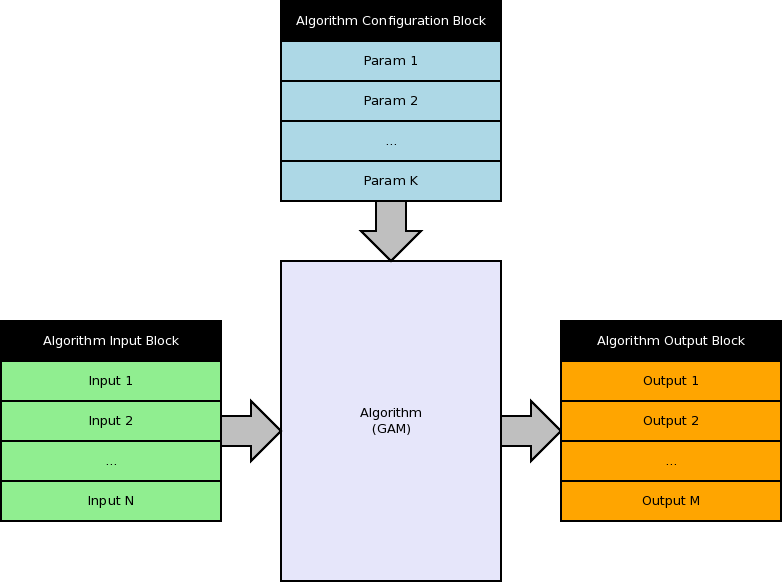
\includegraphics[scale=.33]{GAMs.png}
			\label{fig:gams}
			\caption{GAM}
		\end{figure}
	}
	\only<3>{
		\begin{alertblock}{Warning}
			No interface with operating system (e.g. reading from files/sockets)
		\end{alertblock}
	}
\end{frame}

\begin{frame}[fragile]{Configuration file: GAMs}
	\begin{columns}\column{.8\textwidth}
		\begin{lstlisting}[style=small, language=cfg]
+GAM1 = {
  Class = ExampleGAM
  InputSignals = {
    Input1 = {
      DataSource = DDB1
      Type = uint32
    }
  }
  OutputSignals = {
    Output1 = {
      DataSource = DDB1
      Type = uint32
    }
  }
  Parameters = {
	  Param1 = (uint32) 1000
  }
}\end{lstlisting}
	\end{columns}
\end{frame}

% --- DataSoruces ---
\begin{frame}{Data Sources \& Brokers}
	\begin{block}{Data Sources}
		The \textbf{Data Sources} are the components that provide a interface for the interchange of input and output signals with the memory and the hardware.
	\end{block}
	\begin{block}{Brokers}
		The \textbf{Brokers} are the components that provide the interface between the GAMs memory and the DataSource data.
	\end{block}
	\begin{figure}
		\centering
		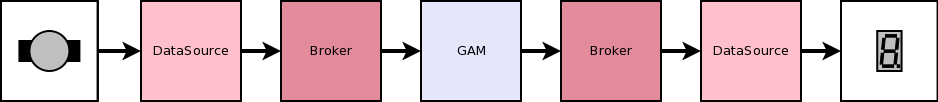
\includegraphics[scale=.35]{DataSources.png}
		\label{fig:datasources}
		\caption{Data Sources \& Brokers}
	\end{figure}
\end{frame}

\begin{frame}[fragile]{Configuration file: Data Sources}
	\begin{columns}\column{.8\textwidth}
		\begin{lstlisting}[style=small, language=cfg]
+Data = { // Data Sources
  Class = ReferenceContainer
  +DDB1 = {
    Class = GAMDataSource
  }
  +Timer = {
    Class = LinuxTimer
    SleepNature = Default
    Signals = {
      Counter = {
	    Type = uint32
	  }
      Time = {
        Type = uint32
      }
    }
	...
  }
}\end{lstlisting}
	\end{columns}
\end{frame}

% --- States ---
\begin{frame}{States}
	\begin{itemize}
		\item \textbg{GAMs} are grouped in real-time \textbg{threads} which are executed in the context of specific \textbg{states}.
		\item A Real-Time application shall be in one (\textbf{and only one}) state at a given time.
	\end{itemize}
\end{frame}
\begin{frame}[fragile]{Configuration file: States}
	\begin{columns}\column{.8\textwidth}
		\begin{lstlisting}[style=small, language=cfg]
+States = { // RT States
  Class = ReferenceContainer
  +State1 = {
    Class = RealTimeState
    +Threads = {
      Class = ReferenceContainer
      +Thread1 = {
        Class = RealTimeThread
        CPUs = 0x8
        Functions = {GAMTimer}
      }
      ...
    }
  }
  ...
}\end{lstlisting}
	\end{columns}
\end{frame}

% --- Scheduler ---
\begin{frame}[fragile]{Configuration file: Scheduler}
	\begin{itemize}
		\item A \textbg{real-time scheduler} handles thread execution;
	\end{itemize}
	\vspace{1cm}
	\begin{columns}\column{.8\textwidth}
		\begin{lstlisting}[style=normal, language=cfg]
+Scheduler = { // Scheduler
  Class = GAMScheduler
  TimingDataSource = Timings
}\end{lstlisting}
	\end{columns}
\end{frame}

% --- RTApp  ---
\begin{frame}{Example: Real-Time Application}
	\begin{figure}
		\centering
		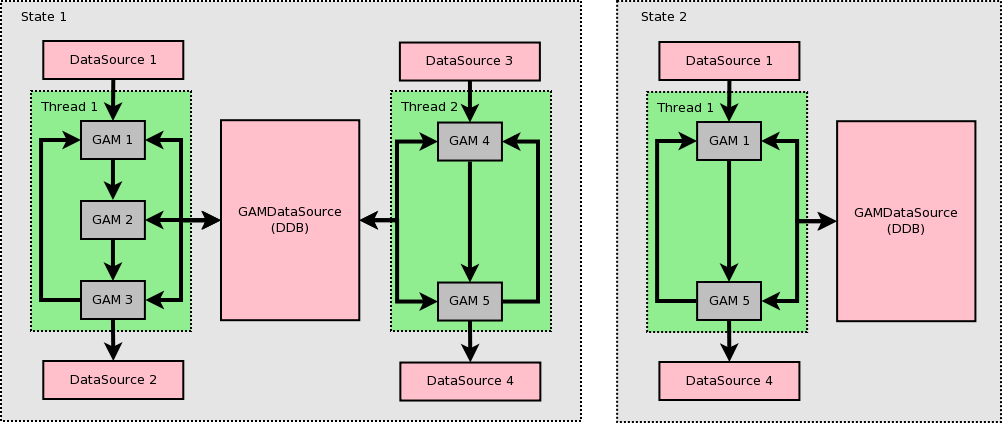
\includegraphics[width=\textwidth]{RTApp.png}
		\label{fig:rtapp_example}
		\caption{Example of a multi-state and multi-threaded real-time application}
	\end{figure}
\end{frame}


% --- Section 4 ---
% Section 4 - StateMachine
% Roberto Masocco <roberto.masocco@uniroma2.it>
% Alessandro Tenaglia <alessandro.tenaglia@uniroma2.it>
% June 5, 2024

% ### StateMachine ###
\section{StateMachine}
\graphicspath{{figs/section4/}}

% --- State Machine ---
\begin{frame}{StateMachine}
  The \textbg{StateMachine} is a software component used to \textbg{synchronize the application states} with the external environment:
	\begin{itemize}
		\item it can be in \textbg{one and only one} state at a given time;
		\item transitions between states are handled by \textbg{Events};
		\item it allows to associate the sending of \textbg{Messages} to \textbg{Events}, \emph{i.e.}, to \textbg{trigger transitions externally}.
	\end{itemize}
	\begin{alertblock}{Warning}
		Be careful not to confuse the states of the \textbr{Real-Time Application} with the states of the \textbr{StateMachine}! The latter is just another software component you can use to implement FSMs.
	\end{alertblock}
\end{frame}

% --- Example: StateMachine ---
\begin{frame}{Example: StateMachine}
	\begin{figure}
		\centering
		\includegraphics[scale=.4]{statemachine.png}
		\caption{Example of StateMachine diagram.}
		\label{fig:statemachine}
	\end{figure}
\end{frame}

% --- Configuration file: StateMachine ---
\begin{frame}[fragile]{Configuration file: StateMachine}
	\begin{columns}\column{.9\textwidth}
		\begin{lstlisting}[style=normal, language=cfg, caption=StateMachine high-level configuration structure (brackets due to space constraints).]
+FSM = { // Declares a StateMachine named FSM
    Class = StateMachine
    +STATE1 = {
        Class = ReferenceContainer
        +GOTOSTATE2 = {
            Class = StateMachineEvent
            ...
        }}
    +STATE2 = {
        Class = ReferenceContainer
        +GOTOSTATE1 = {
            Class = StateMachineEvent
            ...
        }}}\end{lstlisting}
	\end{columns}
\end{frame}

% --- StateMachineEvent ---
\begin{frame}{StateMachineEvent}
	A \textbg{StateMachineEvent} represents a transition and defines:
	\begin{itemize}
		\item \textbg{NextState}, the next state to go to;
		\item \textbg{NextStateError}, the state to go to on error;
		\item one or more \textbg{Messages} to send when each of the following is executed:
		      \begin{itemize}
			      \item \texttt{PrepareNextState}
			      \item \texttt{StopCurrentStateExecution}
			      \item \texttt{StartNextStateExecution}
		      \end{itemize}
	\end{itemize}
\end{frame}

% --- Configuration file: StateMachineEvent ---
\begin{frame}[fragile]{Configuration file: StateMachineEvent}
	\begin{columns}\column{.9\textwidth}
		\begin{lstlisting}[style=normal, language=cfg, caption=StateMachineEvent configuration structure (brackets due to space constraints).]
+GOTOSTATE2 = {
    Class = StateMachineEvent
    NextState = STATE2
    NextStateError = ERROR
    +PrepareChangeToState2Msg = {
        Class = Message
        Function = PrepareNextState}
    +StopCurrentStateExecutionMsg = {
        Class = Message
        Function = StopCurrentStateExecution}
    +StartNextStateExecutionMsg = {
        Class = Message
        Function = StartNextStateExecution}
}\end{lstlisting}
	\end{columns}
\end{frame}


% --- Section 5 ---
% Section 5 - MATLAB
% Alessandro Tenaglia <alessandro.tenaglia@uniroma2.it>
% May 6, 2022

% ### MATLAB ###
\section{MATLAB Coder}
\graphicspath{{figs/section5/}}

% --- Model creation ---
\begin{frame}{Model creation}
	\begin{itemize}
		\item Create the model paying attention to data types;
		\item Define inputs as \textbg{Inport blocks} and name them;
		\item Define outputs as \textbg{Outport blocks} and name them;
	\end{itemize}
	\vspace{0.5cm}
	\begin{figure}
		\centering
		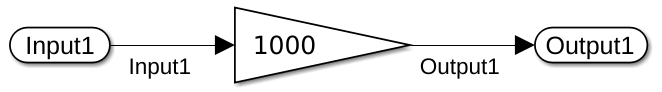
\includegraphics[scale=0.4]{Model.png}
		\label{fig:model}
		\caption{Base model}
	\end{figure}
\end{frame}

% --- Param configuration ---
\begin{frame}{Param configuration}
	Paramters can be:
	\begin{itemize}
		\item \textbg{static}, so no longer modifiable after the code generation;
		\item \textbg{tunable}, so they can be modified at runtime;
	\end{itemize}
	\vspace{0.5cm}
	\begin{figure}
		\centering
		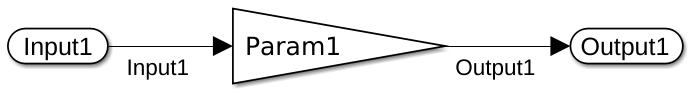
\includegraphics[scale=0.4]{ModelParam.png}
		\label{fig:model_param}
		\caption{Base model with a tunable parameter}
	\end{figure}
\end{frame}

% --- Code generation ---
\begin{frame}{Code generation}
	\begin{figure}
		\centering
		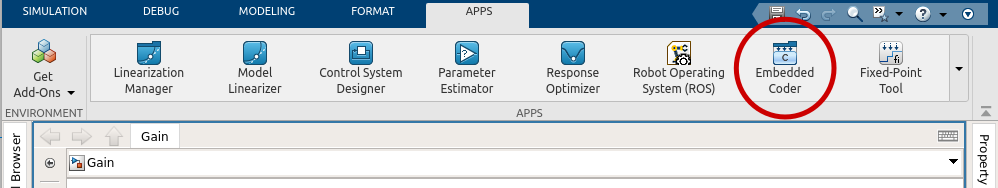
\includegraphics[width=\textwidth]{Embedded.png}
		\label{fig:embedded}
		\caption{Embedded coder app}
	\end{figure}
\end{frame}

% --- Code generation ---
\begin{frame}{Code generation}
	\begin{figure}
		\centering
		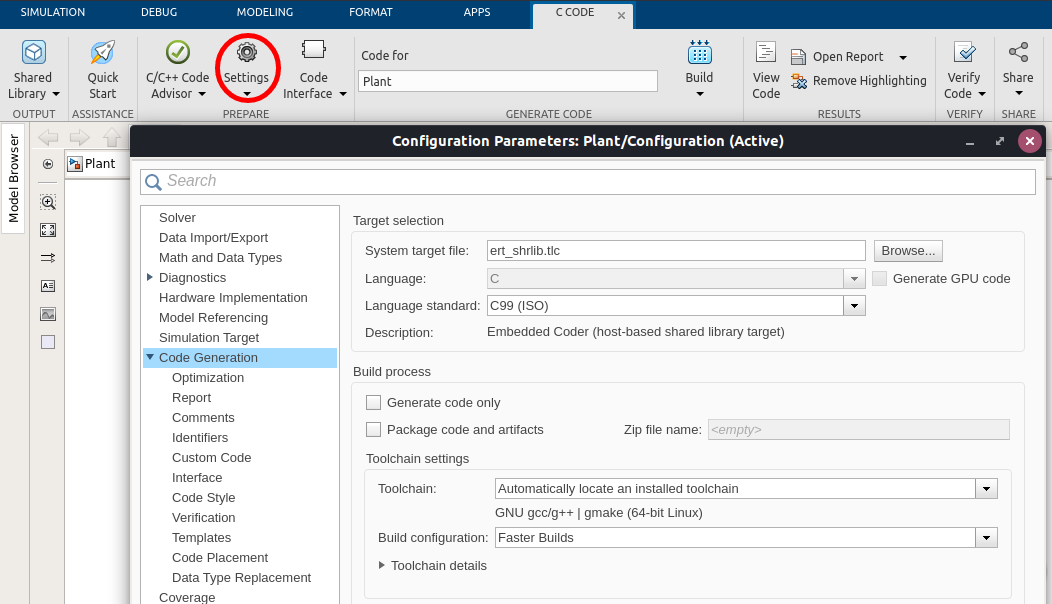
\includegraphics[scale=0.3]{Settings.png}
		\label{fig:settingd}
		\caption{Code generation settings}
	\end{figure}
\end{frame}

% --- Code generation ---
\begin{frame}{Code generation}
	\begin{figure}
		\centering
		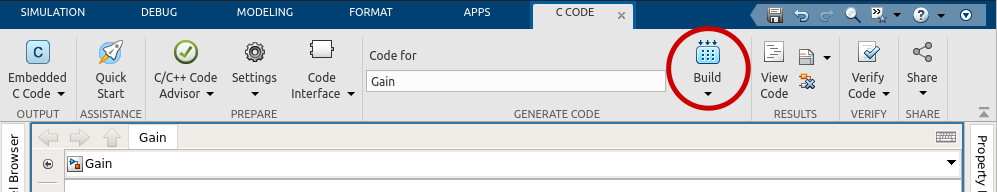
\includegraphics[width=\textwidth]{Build.png}
		\label{fig:build}
		\caption{Base model with tunable parameter}
	\end{figure}
\end{frame}

% --- SimulinkWrapperGAM ---
\begin{frame}[fragile]{Configuration file: SimulinkWrapperGAM}
	\begin{columns}\column{.8\textwidth}
		\begin{lstlisting}[style=small, language = cfg]
+GAMGain = {
    Class = SimulinkWrapperGAM
    Library = Gain.so // Library name
    SymbolPrefix = Gain // Model name
    InputSignals = {
        Input1 = {
            DataSource = DDB1
            Type = int32
        }
    }
    OutputSignals = {
        Output1 = {
            DataSource = DDB1
            Type = int32
        }
    }
    Parameters = {
        Param1 = (int32) 1000
    }
}\end{lstlisting}
	\end{columns}
\end{frame}

% --- Example: Control System ---
\begin{frame}{Example: Control System}
	\begin{figure}
		\centering
		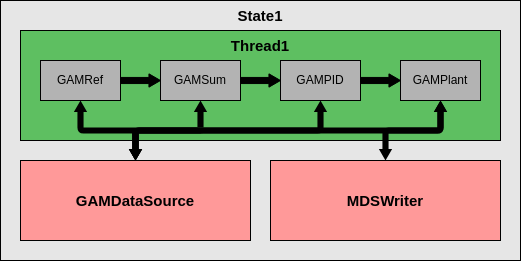
\includegraphics[scale=0.55]{ControlSystem.png}
		\label{fig:control}
		\caption{Control system app scheme}
	\end{figure}
\end{frame}


% --- Section 6 ---
% Section 6 - MDSplus
% Roberto Masocco <roberto.masocco@uniroma2.it>
% Alessandro Tenaglia <alessandro.tenaglia@uniroma2.it>
% June 5, 2024

% ### MDSplus ###
\section{MDSplus}
\graphicspath{{figs/section6/}}

% --- MDSplus ---
\begin{frame}{MDSplus}
	\begin{columns}
		\column{.6\textwidth}
		\textbg{MDSplus} is a tool for \textbg{data acquisition and storage}.\\
    \medskip
		\textbg{MDSplus} stores data in a user-defined hierarchical structure, namely a \textbg{tree}.\\
    \medskip
		A \textbg{tree} is formed by \textbg{nodes}, each of which represents a \textbg{data field}.\\
    \medskip
		Experiments of the same type have the same tree structure and an \textbg{incremental pulse number}.\\
    \medskip
    Trees contents can be inspected with:
    \begin{itemize}
      \item \textbg{jScope} to plot signals;
      \item \textbg{jTraverser} to navigate the tree, inspect nodes and their values;
      \item \textbg{MDSReader}, \textbg{MDSWriter} DataSources.
    \end{itemize}
		\column{.4\textwidth}
		\begin{figure}
			\centering
			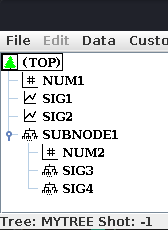
\includegraphics[scale=.5]{tree.png}
			\caption{Example of MDSplus tree\\visualized with jTraverser.}
			\label{fig:tree}
		\end{figure}
	\end{columns}
\end{frame}


\end{document}
